\documentclass[]{book}
\usepackage{lmodern}
\usepackage{amssymb,amsmath}
\usepackage{ifxetex,ifluatex}
\usepackage{fixltx2e} % provides \textsubscript
\ifnum 0\ifxetex 1\fi\ifluatex 1\fi=0 % if pdftex
  \usepackage[T1]{fontenc}
  \usepackage[utf8]{inputenc}
\else % if luatex or xelatex
  \ifxetex
    \usepackage{mathspec}
  \else
    \usepackage{fontspec}
  \fi
  \defaultfontfeatures{Ligatures=TeX,Scale=MatchLowercase}
\fi
% use upquote if available, for straight quotes in verbatim environments
\IfFileExists{upquote.sty}{\usepackage{upquote}}{}
% use microtype if available
\IfFileExists{microtype.sty}{%
\usepackage{microtype}
\UseMicrotypeSet[protrusion]{basicmath} % disable protrusion for tt fonts
}{}
\usepackage[margin=1in]{geometry}
\usepackage{hyperref}
\hypersetup{unicode=true,
            pdftitle={Statistiques et Probabilités avec R et le Tidyverse},
            pdfauthor={Marc-André Désautels},
            pdfborder={0 0 0},
            breaklinks=true}
\urlstyle{same}  % don't use monospace font for urls
\usepackage{natbib}
\bibliographystyle{apalike}
\usepackage{color}
\usepackage{fancyvrb}
\newcommand{\VerbBar}{|}
\newcommand{\VERB}{\Verb[commandchars=\\\{\}]}
\DefineVerbatimEnvironment{Highlighting}{Verbatim}{commandchars=\\\{\}}
% Add ',fontsize=\small' for more characters per line
\usepackage{framed}
\definecolor{shadecolor}{RGB}{248,248,248}
\newenvironment{Shaded}{\begin{snugshade}}{\end{snugshade}}
\newcommand{\KeywordTok}[1]{\textcolor[rgb]{0.13,0.29,0.53}{\textbf{#1}}}
\newcommand{\DataTypeTok}[1]{\textcolor[rgb]{0.13,0.29,0.53}{#1}}
\newcommand{\DecValTok}[1]{\textcolor[rgb]{0.00,0.00,0.81}{#1}}
\newcommand{\BaseNTok}[1]{\textcolor[rgb]{0.00,0.00,0.81}{#1}}
\newcommand{\FloatTok}[1]{\textcolor[rgb]{0.00,0.00,0.81}{#1}}
\newcommand{\ConstantTok}[1]{\textcolor[rgb]{0.00,0.00,0.00}{#1}}
\newcommand{\CharTok}[1]{\textcolor[rgb]{0.31,0.60,0.02}{#1}}
\newcommand{\SpecialCharTok}[1]{\textcolor[rgb]{0.00,0.00,0.00}{#1}}
\newcommand{\StringTok}[1]{\textcolor[rgb]{0.31,0.60,0.02}{#1}}
\newcommand{\VerbatimStringTok}[1]{\textcolor[rgb]{0.31,0.60,0.02}{#1}}
\newcommand{\SpecialStringTok}[1]{\textcolor[rgb]{0.31,0.60,0.02}{#1}}
\newcommand{\ImportTok}[1]{#1}
\newcommand{\CommentTok}[1]{\textcolor[rgb]{0.56,0.35,0.01}{\textit{#1}}}
\newcommand{\DocumentationTok}[1]{\textcolor[rgb]{0.56,0.35,0.01}{\textbf{\textit{#1}}}}
\newcommand{\AnnotationTok}[1]{\textcolor[rgb]{0.56,0.35,0.01}{\textbf{\textit{#1}}}}
\newcommand{\CommentVarTok}[1]{\textcolor[rgb]{0.56,0.35,0.01}{\textbf{\textit{#1}}}}
\newcommand{\OtherTok}[1]{\textcolor[rgb]{0.56,0.35,0.01}{#1}}
\newcommand{\FunctionTok}[1]{\textcolor[rgb]{0.00,0.00,0.00}{#1}}
\newcommand{\VariableTok}[1]{\textcolor[rgb]{0.00,0.00,0.00}{#1}}
\newcommand{\ControlFlowTok}[1]{\textcolor[rgb]{0.13,0.29,0.53}{\textbf{#1}}}
\newcommand{\OperatorTok}[1]{\textcolor[rgb]{0.81,0.36,0.00}{\textbf{#1}}}
\newcommand{\BuiltInTok}[1]{#1}
\newcommand{\ExtensionTok}[1]{#1}
\newcommand{\PreprocessorTok}[1]{\textcolor[rgb]{0.56,0.35,0.01}{\textit{#1}}}
\newcommand{\AttributeTok}[1]{\textcolor[rgb]{0.77,0.63,0.00}{#1}}
\newcommand{\RegionMarkerTok}[1]{#1}
\newcommand{\InformationTok}[1]{\textcolor[rgb]{0.56,0.35,0.01}{\textbf{\textit{#1}}}}
\newcommand{\WarningTok}[1]{\textcolor[rgb]{0.56,0.35,0.01}{\textbf{\textit{#1}}}}
\newcommand{\AlertTok}[1]{\textcolor[rgb]{0.94,0.16,0.16}{#1}}
\newcommand{\ErrorTok}[1]{\textcolor[rgb]{0.64,0.00,0.00}{\textbf{#1}}}
\newcommand{\NormalTok}[1]{#1}
\usepackage{longtable,booktabs}
\usepackage{graphicx,grffile}
\makeatletter
\def\maxwidth{\ifdim\Gin@nat@width>\linewidth\linewidth\else\Gin@nat@width\fi}
\def\maxheight{\ifdim\Gin@nat@height>\textheight\textheight\else\Gin@nat@height\fi}
\makeatother
% Scale images if necessary, so that they will not overflow the page
% margins by default, and it is still possible to overwrite the defaults
% using explicit options in \includegraphics[width, height, ...]{}
\setkeys{Gin}{width=\maxwidth,height=\maxheight,keepaspectratio}
\IfFileExists{parskip.sty}{%
\usepackage{parskip}
}{% else
\setlength{\parindent}{0pt}
\setlength{\parskip}{6pt plus 2pt minus 1pt}
}
\setlength{\emergencystretch}{3em}  % prevent overfull lines
\providecommand{\tightlist}{%
  \setlength{\itemsep}{0pt}\setlength{\parskip}{0pt}}
\setcounter{secnumdepth}{5}
% Redefines (sub)paragraphs to behave more like sections
\ifx\paragraph\undefined\else
\let\oldparagraph\paragraph
\renewcommand{\paragraph}[1]{\oldparagraph{#1}\mbox{}}
\fi
\ifx\subparagraph\undefined\else
\let\oldsubparagraph\subparagraph
\renewcommand{\subparagraph}[1]{\oldsubparagraph{#1}\mbox{}}
\fi

%%% Use protect on footnotes to avoid problems with footnotes in titles
\let\rmarkdownfootnote\footnote%
\def\footnote{\protect\rmarkdownfootnote}

%%% Change title format to be more compact
\usepackage{titling}

% Create subtitle command for use in maketitle
\newcommand{\subtitle}[1]{
  \posttitle{
    \begin{center}\large#1\end{center}
    }
}

\setlength{\droptitle}{-2em}
  \title{Statistiques et Probabilités avec R et le Tidyverse}
  \pretitle{\vspace{\droptitle}\centering\huge}
  \posttitle{\par}
  \author{Marc-André Désautels}
  \preauthor{\centering\large\emph}
  \postauthor{\par}
  \predate{\centering\large\emph}
  \postdate{\par}
  \date{2018-04-04}

\usepackage{booktabs}

\begin{document}
\maketitle

{
\setcounter{tocdepth}{1}
\tableofcontents
}
\chapter*{Introduction}\label{introduction}
\addcontentsline{toc}{chapter}{Introduction}

\part{Pourquoi le
tidyverse}\label{part-pourquoi-le-tidyverse}

\chapter{Le tidyverse}\label{tidyverse}

Dans ce document, nous utiliserons l'extension \texttt{tidyverse} par
\citep{R-tidyverse}. Ce chapitre permettra d'introduire l'extension
\texttt{tidyverse} mais surtout les principes qui la sous-tendent. Ce
chapitre est inspiré de \citep{juba2018} et \citep{wickham2017}.

\section{Extensions}\label{extensions}

Le terme \emph{tidyverse} est une contraction de \emph{tidy} (qu'on
pourrait traduire par ``bien rangé'') et de \emph{universe}. En allant
visiter le site internet de ces extensions
\url{https://www.tidyverse.org/}, voici ce que nous pouvons trouver sur
la première page du site:

\begin{quote}
The tidyverse is an opinionated collection of R packages designed for
data science. All packages share an underlying design philosophy,
grammar, and data structures.
\end{quote}

que nous pourrions traduire par:

\begin{quote}
Le tidyverse est une collection dogmatique d'extensions pour le langage
R conçues pour la science des données. Toutes les extensions partagent
une philosphie sous-jacente de design, de grammaire et de structures de
données.
\end{quote}

Ces extensions abordent un très grand nombre d'opérations courantes dans
\texttt{R}. L'avantage d'utiliser le \texttt{tidyverse} c'est qu'il
permet de simplifier plusieurs opérations fréquentes et il introduit le
concept de \textbf{tidy data}. De plus, la grammaire du
\texttt{tidyverse} étant cohérente entre toutes ses extensions, en
apprenant comment utiliser l'une de ces extensions, vous serez en monde
connu lorsque viendra le temps d'apprendre de nouvelles extensions.

Nous utiliserons le \texttt{tidyverse} pour:

\begin{itemize}
\tightlist
\item
  Le concept de \textbf{tidy data}
\item
  L'importation et/ou l'exportation de données
\item
  La manipulation de variables
\item
  La visualisation
\end{itemize}

Le \texttt{tidyverse} permet aussi de:

\begin{itemize}
\tightlist
\item
  Travailler avec des chaînes de caractères (du texte par exemple)
\item
  Programmer
\item
  Remettre en forme des données
\item
  Extraire des données du Web
\item
  Etc.
\end{itemize}

Pour en savoir plus, nous invitons le lecteur à se rendre au site du
\texttt{tidyverse} \url{https://www.tidyverse.org/}. Le
\texttt{tidyverse} est en grande partie issu des travaux de
\href{http://hadley.nz/}{Hadley Wickham}.

\section{Installation}\label{installation}

Pour installer les extensions du \texttt{tidyverse}, nous effectuons la
commande suivante:

\begin{Shaded}
\begin{Highlighting}[]
\KeywordTok{install.packages}\NormalTok{(}\StringTok{"tidyverse"}\NormalTok{)}
\end{Highlighting}
\end{Shaded}

Une fois l'extension installée, il n'est pas nécessaire de la
réinstaller à chaque fois que vous utilisez \texttt{R}. Par contre, vous
devez charger l'extension à chaque fois que vous utilisez \texttt{R}.

Pour charger l'extension et l'utiliser dans \texttt{R}, nous effectuons
la commande suivante:

\begin{Shaded}
\begin{Highlighting}[]
\KeywordTok{library}\NormalTok{(tidyverse)}
\end{Highlighting}
\end{Shaded}

Cette commande va en fait charger plusieurs extensions qui constituent
le \textbf{coeur} du \texttt{tidyverse}, à savoir :

\begin{itemize}
\tightlist
\item
  \texttt{ggplot2} (visualisation)
\item
  \texttt{dplyr} (manipulation des données)
\item
  \texttt{tidyr} (remise en forme des données)
\item
  \texttt{purrr} (programmation)
\item
  \texttt{readr} (importation de données)
\item
  \texttt{tibble} (tableaux de données)
\item
  \texttt{forcats} (variables qualitatives)
\item
  \texttt{stringr} (chaînes de caractères)
\end{itemize}

Il existe d'autres extensions qui font partie du \texttt{tidyverse} mais
qui doivent être chargées explicitement, comme par exemple
\texttt{readxl} (pour l'importation de données depuis des fichiers
Excel).

La liste complète des extensions se trouve sur le site officiel du
\texttt{tidyverse} \url{https://www.tidyverse.org/packages/}.

\section{Les tidy data}\label{tidydata}

Le \texttt{tidyverse} est en partie fondé sur le concept de \emph{tidy
data}, développé à l'origine par Hadley Wickham dans un article du
\emph{Journal of Statistical Software}, voir \citep{wickham2014}. Nous
pourrions traduire ce concept par \emph{données bien rangées}.

Il s'agit d'un modèle d'organisation des données qui vise à faciliter le
travail souvent long et fastidieux de nettoyage et de préparation
préalable à la mise en oeuvre de méthodes d'analyse. Dans ce livre, nous
travaillerons toujours avec des \emph{tidy data}. En réalité, la plupart
des données rencontrées par les chercheurs ne sont pas \emph{tidy}. Il
existe une extension du \texttt{tidyverse} qui permet de faciliter la
transformation de données \emph{non tidy} en données \emph{tidy},
l'extension \texttt{tidyr}. Nous ne verrons pas comment l'utiliser dans
ce livre.

Les principes d'un jeu de données \emph{tidy} sont les suivants :

\begin{enumerate}
\def\labelenumi{\arabic{enumi}.}
\tightlist
\item
  chaque variable est une colonne
\item
  chaque observation est une ligne
\item
  chaque valeur doit être dans une cellule différente
\end{enumerate}

La figure \ref{fig:tidy-structure} montre ces règles de façon visuelle
(l'image a été prise de \citep{wickham2017}).

\begin{figure}

{\centering 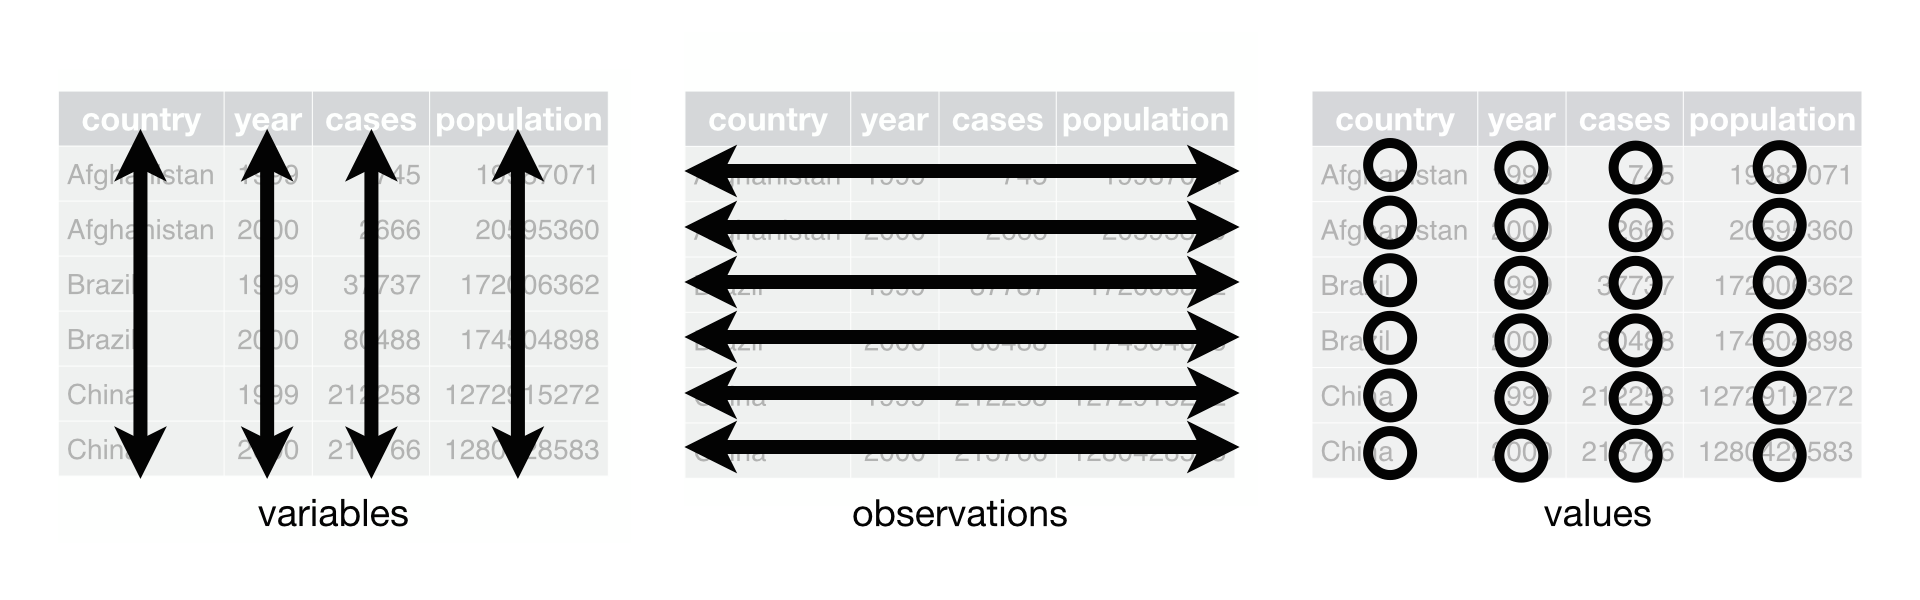
\includegraphics[width=1\linewidth]{images/tidy-1} 

}

\caption{Suivre les trois principes rend les données tidy: les variables sont en colonnes, les observations sont sur des lignes, et chaques valeurs sont dans des cellules différentes.}\label{fig:tidy-structure}
\end{figure}

Pourquoi s'assurer que vos données sont \emph{tidy}? Il y a deux
avantages importants:

\begin{enumerate}
\def\labelenumi{\arabic{enumi}.}
\item
  Un avantage général de choisir une seule façon de conserver vos
  données. Si vous utilisez une structure de données consitante, il est
  plus facile d'apprendre à utiliser les outils qui fonctionneront avec
  ce type de structure, étant donné que celles-ci possède une uniformité
  sous-jacente.
\item
  Un avantage spécifique de placer les variables en colonnes car ceci
  permet de \emph{vectoriser} les opérations dans \texttt{R}. Ceci
  implique que vos fonctions seront plus rapides lorsque viendra le
  temps de les exécuter.
\end{enumerate}

Voici un exemple de données \emph{tidy} qui sont accessibles en
\texttt{R} de base.

\begin{Shaded}
\begin{Highlighting}[]
\KeywordTok{as_tibble}\NormalTok{(}\KeywordTok{rownames_to_column}\NormalTok{(mtcars))}
\end{Highlighting}
\end{Shaded}

\begin{verbatim}
## # A tibble: 32 x 12
##   rowname        mpg   cyl  disp    hp  drat    wt  qsec    vs    am  gear
##   <chr>        <dbl> <dbl> <dbl> <dbl> <dbl> <dbl> <dbl> <dbl> <dbl> <dbl>
## 1 Mazda RX4     21.0    6.  160.  110.  3.90  2.62  16.5    0.    1.    4.
## 2 Mazda RX4 W~  21.0    6.  160.  110.  3.90  2.88  17.0    0.    1.    4.
## 3 Datsun 710    22.8    4.  108.   93.  3.85  2.32  18.6    1.    1.    4.
## 4 Hornet 4 Dr~  21.4    6.  258.  110.  3.08  3.22  19.4    1.    0.    3.
## 5 Hornet Spor~  18.7    8.  360.  175.  3.15  3.44  17.0    0.    0.    3.
## 6 Valiant       18.1    6.  225.  105.  2.76  3.46  20.2    1.    0.    3.
## # ... with 26 more rows, and 1 more variable: carb <dbl>
\end{verbatim}

\section{Les tibbles}\label{tibbles}

Une autre particularité du \emph{tidyverse} est que ces extensions
travaillent avec des tableaux de données au format \emph{tibble}, qui
est une évolution plus moderne du classique \emph{data frame} du R de
base. Ce format est fourni est géré par l'extension du même nom
(\texttt{tibble}), qui fait partie du coeur du \emph{tidyverse}. La
plupart des fonctions des extensions du \emph{tidyverse} acceptent des
\emph{data frames} en entrée, mais retournent un objet de classe
\texttt{tibble}.

Contrairement aux \emph{data frames}, les \emph{tibbles} :

\begin{itemize}
\tightlist
\item
  n'ont pas de noms de lignes (\emph{rownames})
\item
  autorisent des noms de colonnes invalides pour les \emph{data frames}
  (espaces, caractères spéciaux, nombres\ldots{}) \footnote{Quand on
    veut utiliser des noms de ce type, on doit les entourer avec des
    \emph{backticks} (`)}
\item
  s'affichent plus intelligemment que les \emph{data frames} : seules
  les premières lignes sont affichées, ainsi que quelques informations
  supplémentaires utiles (dimensions, types des colonnes\ldots{})
\item
  ne font pas de \emph{partial matching} sur les noms de colonnes
  \footnote{Dans R de base, si une table \texttt{d} contient une colonne
    \texttt{qualif}, \texttt{d\$qual} retournera cette colonne.}
\item
  affichent un avertissement si on essaie d'accéder à une colonne qui
  n'existe pas
\end{itemize}

Pour autant, les tibbles restent compatibles avec les \emph{data
frames}. On peut ainsi facilement convertir un \emph{data frame} en
tibble avec \texttt{as\_tibble} :

\begin{Shaded}
\begin{Highlighting}[]
\KeywordTok{as_tibble}\NormalTok{(mtcars)}
\end{Highlighting}
\end{Shaded}

\begin{verbatim}
## # A tibble: 32 x 11
##     mpg   cyl  disp    hp  drat    wt  qsec    vs    am  gear  carb
## * <dbl> <dbl> <dbl> <dbl> <dbl> <dbl> <dbl> <dbl> <dbl> <dbl> <dbl>
## 1  21.0    6.  160.  110.  3.90  2.62  16.5    0.    1.    4.    4.
## 2  21.0    6.  160.  110.  3.90  2.88  17.0    0.    1.    4.    4.
## 3  22.8    4.  108.   93.  3.85  2.32  18.6    1.    1.    4.    1.
## 4  21.4    6.  258.  110.  3.08  3.22  19.4    1.    0.    3.    1.
## 5  18.7    8.  360.  175.  3.15  3.44  17.0    0.    0.    3.    2.
## 6  18.1    6.  225.  105.  2.76  3.46  20.2    1.    0.    3.    1.
## # ... with 26 more rows
\end{verbatim}

Si le \emph{data frame} d'origine a des \emph{rownames}, on peut d'abord
les convertir en colonnes avec \texttt{rownames\_to\_columns} :

\begin{Shaded}
\begin{Highlighting}[]
\NormalTok{d <-}\StringTok{ }\KeywordTok{as_tibble}\NormalTok{(}\KeywordTok{rownames_to_column}\NormalTok{(mtcars))}
\NormalTok{d}
\end{Highlighting}
\end{Shaded}

\begin{verbatim}
## # A tibble: 32 x 12
##   rowname        mpg   cyl  disp    hp  drat    wt  qsec    vs    am  gear
##   <chr>        <dbl> <dbl> <dbl> <dbl> <dbl> <dbl> <dbl> <dbl> <dbl> <dbl>
## 1 Mazda RX4     21.0    6.  160.  110.  3.90  2.62  16.5    0.    1.    4.
## 2 Mazda RX4 W~  21.0    6.  160.  110.  3.90  2.88  17.0    0.    1.    4.
## 3 Datsun 710    22.8    4.  108.   93.  3.85  2.32  18.6    1.    1.    4.
## 4 Hornet 4 Dr~  21.4    6.  258.  110.  3.08  3.22  19.4    1.    0.    3.
## 5 Hornet Spor~  18.7    8.  360.  175.  3.15  3.44  17.0    0.    0.    3.
## 6 Valiant       18.1    6.  225.  105.  2.76  3.46  20.2    1.    0.    3.
## # ... with 26 more rows, and 1 more variable: carb <dbl>
\end{verbatim}

À l'inverse, on peut à tout moment convertir un tibble en \emph{data
frame} avec \texttt{as.data.frame} :

\begin{Shaded}
\begin{Highlighting}[]
\KeywordTok{as.data.frame}\NormalTok{(d)}
\end{Highlighting}
\end{Shaded}

\begin{verbatim}
##                rowname  mpg cyl  disp  hp drat   wt qsec vs am gear carb
## 1            Mazda RX4 21.0   6 160.0 110 3.90 2.62 16.5  0  1    4    4
## 2        Mazda RX4 Wag 21.0   6 160.0 110 3.90 2.88 17.0  0  1    4    4
## 3           Datsun 710 22.8   4 108.0  93 3.85 2.32 18.6  1  1    4    1
## 4       Hornet 4 Drive 21.4   6 258.0 110 3.08 3.21 19.4  1  0    3    1
## 5    Hornet Sportabout 18.7   8 360.0 175 3.15 3.44 17.0  0  0    3    2
## 6              Valiant 18.1   6 225.0 105 2.76 3.46 20.2  1  0    3    1
## 7           Duster 360 14.3   8 360.0 245 3.21 3.57 15.8  0  0    3    4
## 8            Merc 240D 24.4   4 146.7  62 3.69 3.19 20.0  1  0    4    2
## 9             Merc 230 22.8   4 140.8  95 3.92 3.15 22.9  1  0    4    2
## 10            Merc 280 19.2   6 167.6 123 3.92 3.44 18.3  1  0    4    4
## 11           Merc 280C 17.8   6 167.6 123 3.92 3.44 18.9  1  0    4    4
## 12          Merc 450SE 16.4   8 275.8 180 3.07 4.07 17.4  0  0    3    3
## 13          Merc 450SL 17.3   8 275.8 180 3.07 3.73 17.6  0  0    3    3
## 14         Merc 450SLC 15.2   8 275.8 180 3.07 3.78 18.0  0  0    3    3
## 15  Cadillac Fleetwood 10.4   8 472.0 205 2.93 5.25 18.0  0  0    3    4
## 16 Lincoln Continental 10.4   8 460.0 215 3.00 5.42 17.8  0  0    3    4
## 17   Chrysler Imperial 14.7   8 440.0 230 3.23 5.34 17.4  0  0    3    4
## 18            Fiat 128 32.4   4  78.7  66 4.08 2.20 19.5  1  1    4    1
## 19         Honda Civic 30.4   4  75.7  52 4.93 1.61 18.5  1  1    4    2
## 20      Toyota Corolla 33.9   4  71.1  65 4.22 1.83 19.9  1  1    4    1
## 21       Toyota Corona 21.5   4 120.1  97 3.70 2.46 20.0  1  0    3    1
## 22    Dodge Challenger 15.5   8 318.0 150 2.76 3.52 16.9  0  0    3    2
## 23         AMC Javelin 15.2   8 304.0 150 3.15 3.44 17.3  0  0    3    2
## 24          Camaro Z28 13.3   8 350.0 245 3.73 3.84 15.4  0  0    3    4
## 25    Pontiac Firebird 19.2   8 400.0 175 3.08 3.85 17.1  0  0    3    2
## 26           Fiat X1-9 27.3   4  79.0  66 4.08 1.94 18.9  1  1    4    1
## 27       Porsche 914-2 26.0   4 120.3  91 4.43 2.14 16.7  0  1    5    2
## 28        Lotus Europa 30.4   4  95.1 113 3.77 1.51 16.9  1  1    5    2
## 29      Ford Pantera L 15.8   8 351.0 264 4.22 3.17 14.5  0  1    5    4
## 30        Ferrari Dino 19.7   6 145.0 175 3.62 2.77 15.5  0  1    5    6
## 31       Maserati Bora 15.0   8 301.0 335 3.54 3.57 14.6  0  1    5    8
## 32          Volvo 142E 21.4   4 121.0 109 4.11 2.78 18.6  1  1    4    2
\end{verbatim}

Là encore, on peut convertir la colonne \texttt{rowname} en ``vrais''
\emph{rownames} avec \texttt{column\_to\_rownames} :

\begin{Shaded}
\begin{Highlighting}[]
\KeywordTok{column_to_rownames}\NormalTok{(}\KeywordTok{as.data.frame}\NormalTok{(d))}
\end{Highlighting}
\end{Shaded}

\begin{verbatim}
##                      mpg cyl  disp  hp drat   wt qsec vs am gear carb
## Mazda RX4           21.0   6 160.0 110 3.90 2.62 16.5  0  1    4    4
## Mazda RX4 Wag       21.0   6 160.0 110 3.90 2.88 17.0  0  1    4    4
## Datsun 710          22.8   4 108.0  93 3.85 2.32 18.6  1  1    4    1
## Hornet 4 Drive      21.4   6 258.0 110 3.08 3.21 19.4  1  0    3    1
## Hornet Sportabout   18.7   8 360.0 175 3.15 3.44 17.0  0  0    3    2
## Valiant             18.1   6 225.0 105 2.76 3.46 20.2  1  0    3    1
## Duster 360          14.3   8 360.0 245 3.21 3.57 15.8  0  0    3    4
## Merc 240D           24.4   4 146.7  62 3.69 3.19 20.0  1  0    4    2
## Merc 230            22.8   4 140.8  95 3.92 3.15 22.9  1  0    4    2
## Merc 280            19.2   6 167.6 123 3.92 3.44 18.3  1  0    4    4
## Merc 280C           17.8   6 167.6 123 3.92 3.44 18.9  1  0    4    4
## Merc 450SE          16.4   8 275.8 180 3.07 4.07 17.4  0  0    3    3
## Merc 450SL          17.3   8 275.8 180 3.07 3.73 17.6  0  0    3    3
## Merc 450SLC         15.2   8 275.8 180 3.07 3.78 18.0  0  0    3    3
## Cadillac Fleetwood  10.4   8 472.0 205 2.93 5.25 18.0  0  0    3    4
## Lincoln Continental 10.4   8 460.0 215 3.00 5.42 17.8  0  0    3    4
## Chrysler Imperial   14.7   8 440.0 230 3.23 5.34 17.4  0  0    3    4
## Fiat 128            32.4   4  78.7  66 4.08 2.20 19.5  1  1    4    1
## Honda Civic         30.4   4  75.7  52 4.93 1.61 18.5  1  1    4    2
## Toyota Corolla      33.9   4  71.1  65 4.22 1.83 19.9  1  1    4    1
## Toyota Corona       21.5   4 120.1  97 3.70 2.46 20.0  1  0    3    1
## Dodge Challenger    15.5   8 318.0 150 2.76 3.52 16.9  0  0    3    2
## AMC Javelin         15.2   8 304.0 150 3.15 3.44 17.3  0  0    3    2
## Camaro Z28          13.3   8 350.0 245 3.73 3.84 15.4  0  0    3    4
## Pontiac Firebird    19.2   8 400.0 175 3.08 3.85 17.1  0  0    3    2
## Fiat X1-9           27.3   4  79.0  66 4.08 1.94 18.9  1  1    4    1
## Porsche 914-2       26.0   4 120.3  91 4.43 2.14 16.7  0  1    5    2
## Lotus Europa        30.4   4  95.1 113 3.77 1.51 16.9  1  1    5    2
## Ford Pantera L      15.8   8 351.0 264 4.22 3.17 14.5  0  1    5    4
## Ferrari Dino        19.7   6 145.0 175 3.62 2.77 15.5  0  1    5    6
## Maserati Bora       15.0   8 301.0 335 3.54 3.57 14.6  0  1    5    8
## Volvo 142E          21.4   4 121.0 109 4.11 2.78 18.6  1  1    4    2
\end{verbatim}

\begin{rmdnote}
Les deux fonctions \texttt{column\_to\_rownames} et
\texttt{rownames\_to\_column} acceptent un argument supplémentaire
\texttt{var} qui permet d'indiquer un nom de colonne autre que le nom
\texttt{rowname} utilisé par défaut pour créer ou identifier la colonne
contenant les noms de lignes.
\end{rmdnote}

\chapter{Les types de variables}\label{typesvariables}

\chapter{Les types de représentation graphiques}\label{graphiques}

\chapter{Les différentes mesures}\label{mesures}

\bibliography{book.bib,packages.bib}


\end{document}
